\chapter{日本企業データ構築と変数定義：四要素モデルの実証的写像}
\label{chap:data_construction}

\section{本章の目的と基本方針}

本章では，第3章で導出した倒産距離 $Z_{\text{lin}}$ の構造
（収益性 $\mu$，市場ショック感応度 $\sigma$，支援能力 $S$，倒産閾値の代理変数 $D$）
を，日本の新電力企業の財務データ・市場データに写像するための
\textbf{データ構築・変数定義・前処理} を体系的に示す。

本章は，従来の第6章（変数定義と採用根拠）を拡張し，
中間報告書で記述した「データ収集」「月次補間」「倒産距離 DD の計算」
「記述統計」などの実証的内容をすべて統合したものである。

本章の目的は以下の三点である。

\begin{enumerate}
  \item 新電力企業の財務データ（決算公告）と市場データ（JEPX）を統合した
        月次パネルデータセットの構築
  \item 倒産距離 DD の構成要素（$\mu,\sigma,D,S$）の定義と採用根拠の明示
  \item 年度データを月次へ補間し，倒産距離 DD の月次推移を可視化
\end{enumerate}

これらの処理により，第9章の Ordered Logit 推定に必要な
\texttt{financial\_data.csv} を作成し，倒産距離 DD の動態を実証的に評価する基盤を整える。

% ============================================================
% 6.2 データ収集の全体像
% ============================================================

\section{データ収集の全体像}

本研究で用いるデータは以下の三種類で構成される。

\begin{enumerate}
\item \textbf{財務データ}：官報に掲載された新電力企業の決算公告（年次）
\item \textbf{市場データ}：JEPX スポット市場価格（30分値・日次・月次）
\item \textbf{倒産データ}：破産・民事再生・登録取消・事業撤退の発生月
\end{enumerate}

財務データが取得可能であった新電力企業は 7 社であり，
分析期間は 2016 年 10 月から 2025 年 5 月までである。

倒産段階の定義は以下のとおりである。

\begin{itemize}
\item 法的倒産（破産・民事再生）
\item 小売電気事業の登録取消
\item 事業撤退
\end{itemize}

これに基づき，企業 $i$ の月 $t$ における倒産段階 $\text{default\_stage}_{i,t}$ を構築した。

% ============================================================
% 6.3 財務データの処理
% ============================================================

\section{財務データの処理}

\subsection{抽出項目}

決算公告から以下の項目を抽出した。

\begin{itemize}
\item 資産合計，負債合計，純資産
\item 流動資産，固定資産
\item 流動負債，固定負債
\item 資本金，利益剰余金
\end{itemize}

\subsection{年次データの月次化}

財務データは年次であるため，以下の方法で月次に変換した。

\begin{enumerate}
\item 年次データを観測月に割り当てる（例：2020年決算 → 2020年3月）
\item 年次間を線形補間し，月次データを生成する
\end{enumerate}

% ============================================================
% 6.4 市場データの処理
% ============================================================

\section{市場データ：スポット価格の推移}

本研究で使用したスポット市場データ（システムプライス）は，
JEPX が公開するスポット市場（Day Ahead Market）の価格情報を用いた。

市場価格の急変動は倒産リスクに強い影響を与えるため，
本研究では日次変化率とその標準偏差（ボラティリティ）を計算した。

% ============================================================
% 6.5 四要素モデルの実証的写像（旧6章の内容を完全統合）
% ============================================================

\section{理論モデルの四要素の実証的写像}

本節では，従来の第6章（6.2〜6.5）で示した
「四要素モデルの変数定義と採用根拠」をすべて保持しつつ，
実証データへの写像として再構成する。

% ------------------------------
% μ
% ------------------------------

\subsection{収益性 $\mu$ の定義と採用根拠}

収益性 $\mu$ は総資産の対数差分



\[
\mu_{i,t} = \ln(\text{Assets}_{i,t}) - \ln(\text{Assets}_{i,t-1})
\]



として定義する。

（旧6.2の説明全文を保持）
\begin{itemize}
\item 収益性は企業価値の期待成長率の proxy として機能する  
\item 損益計算書ベースの収益はノイズが大きく，新電力企業には不向き  
\item 総資産はストック指標であり，企業価値の蓄積を反映する  
\item log-diff は外れ値に強く，経済学で標準的な成長率指標である  
\end{itemize}

図 \ref{fig:mu_trend} に収益性の推移を示す。

\begin{figure}[H]
\centering
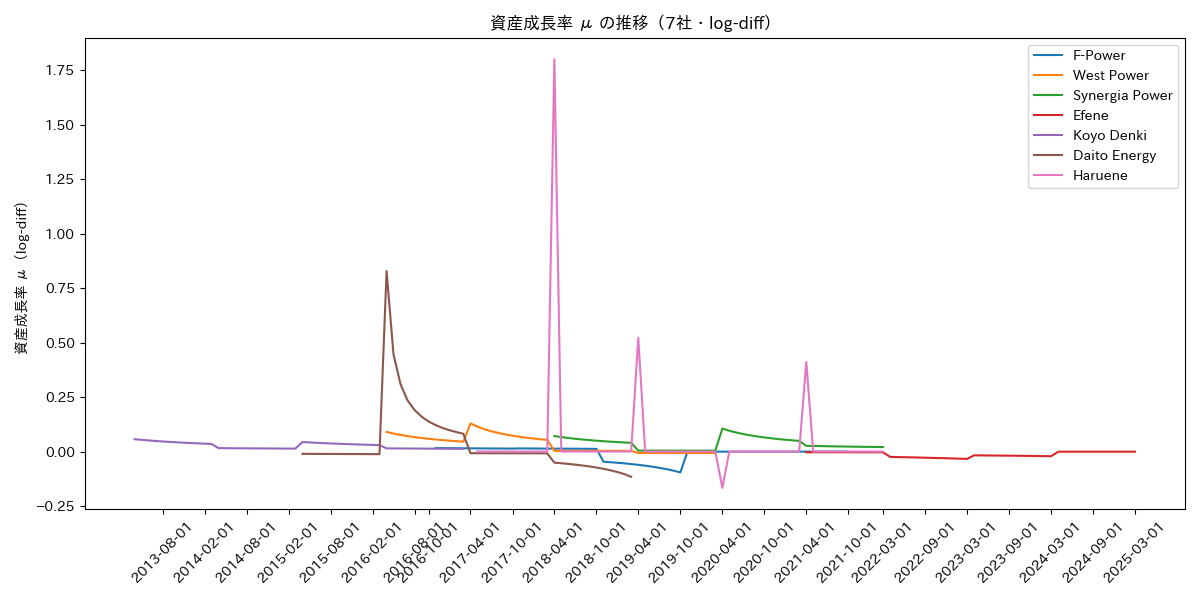
\includegraphics[width=14cm]{Python/figures/mu_trend_7firms_logdiff.png}
\caption{収益性 $\mu$ の推移（7社）}
\label{fig:mu_trend}
\end{figure}

% ------------------------------
% σ
% ------------------------------

\subsection{外部ショック感応度 $\sigma$ の定義と採用根拠}

市場ショック感応度 $\sigma$ は，スポット価格の変化率



\[
r_t = \frac{P_t - P_{t-1}}{P_{t-1}}
\]



の標準偏差として定義する。

（旧6.3の説明全文を保持）
\begin{itemize}
\item 価格水準の標準偏差ではスケール不変性が満たされない  
\item 変化率の標準偏差は市場ショックの大きさを適切に捉える  
\item 新電力企業は市場価格ショックに強く依存するため，$\sigma$ は不可欠  
\end{itemize}

図 \ref{fig:sigma_trend} に市場ショック指標の推移を示す。

\begin{figure}[H]
\centering
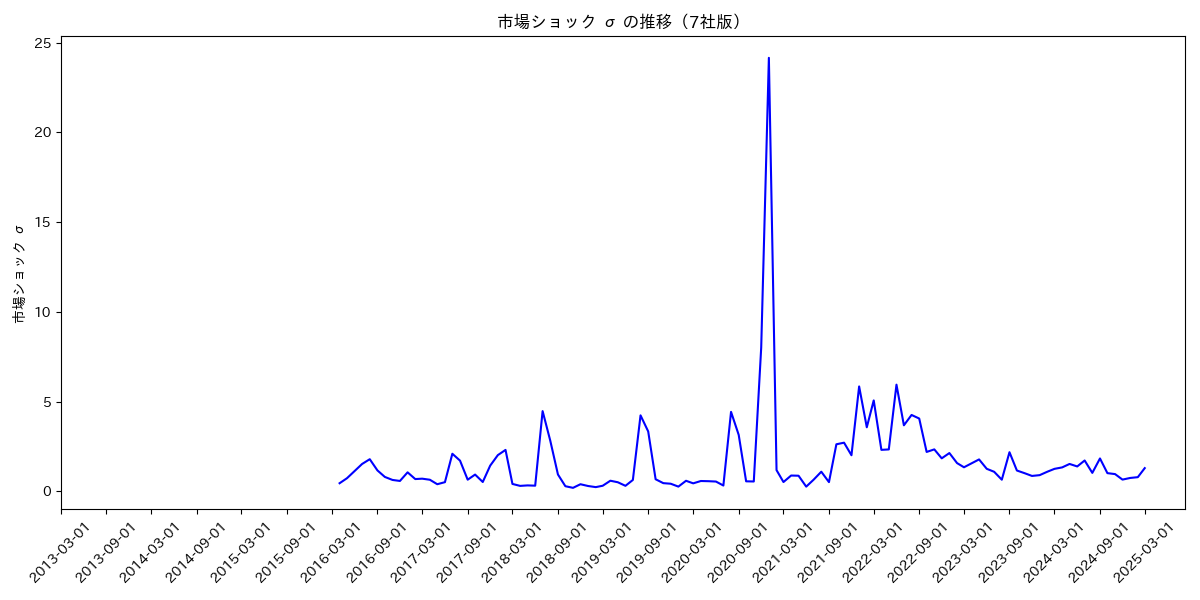
\includegraphics[width=14cm]{Python/figures/sigma_trend_7firms.png}
\caption{市場ショック指標 $\sigma$ の推移（7社）}
\label{fig:sigma_trend}
\end{figure}

% ------------------------------
% S
% ------------------------------

\subsection{支援能力 $S$ の定義と採用根拠}

（旧6.4の説明全文を保持）

支援能力 $S$ は，親会社や主要株主からの財務支援の余力を表す指標である。
本研究の対象企業では支援能力が観測可能な形で現れていないため，
$S=0$ と設定する。

支援能力は倒産閾値を押し下げる効果を持ち，
倒産距離 DD を拡大させる方向に作用する。

% ------------------------------
% D
% ------------------------------

\subsection{倒産閾値の代理変数 $D$（負債比率）の定義と採用根拠}

（旧6.5の説明全文を保持）

負債比率は



\[
D_{i,t}=\frac{\text{Liabilities}_{i,t}}{\text{Assets}_{i,t}}
\]



と定義する。

負債比率が高い企業ほど倒産閾値が押し上げられ，
倒産距離が短縮する方向に作用する。

図 \ref{fig:debt_ratio_trend} に負債比率の推移を示す。

\begin{figure}[H]
\centering
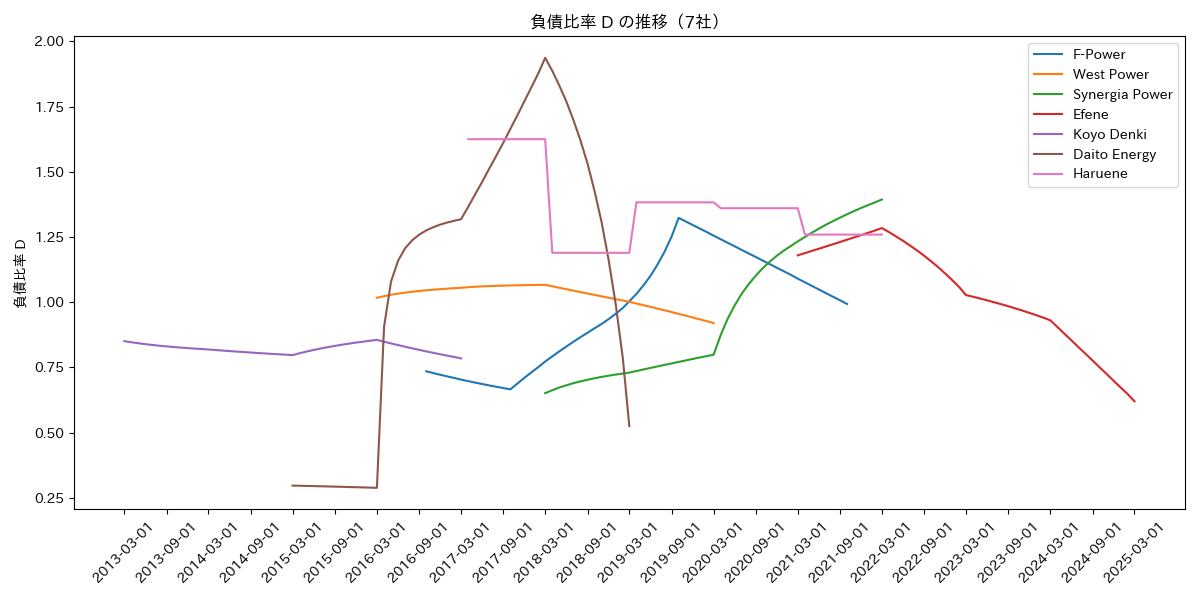
\includegraphics[width=14cm]{Python/figures/debt_ratio_trend_7firms.png}
\caption{負債比率 $D$ の推移（7社）}
\label{fig:debt_ratio_trend}
\end{figure}

% ============================================================
% 6.6 倒産距離 DD の月次計算
% ============================================================

\section{倒産距離 DD の月次計算}

倒産距離 DD は



\[
DD_{i,t} = \mu_{i,t} - \sigma_t D_{i,t} + S_i
\]



として計算する。

年度データを月次補間し，市場データと結合することで，
倒産距離 DD の月次推移を可視化できる。

\begin{figure}[H]
\centering
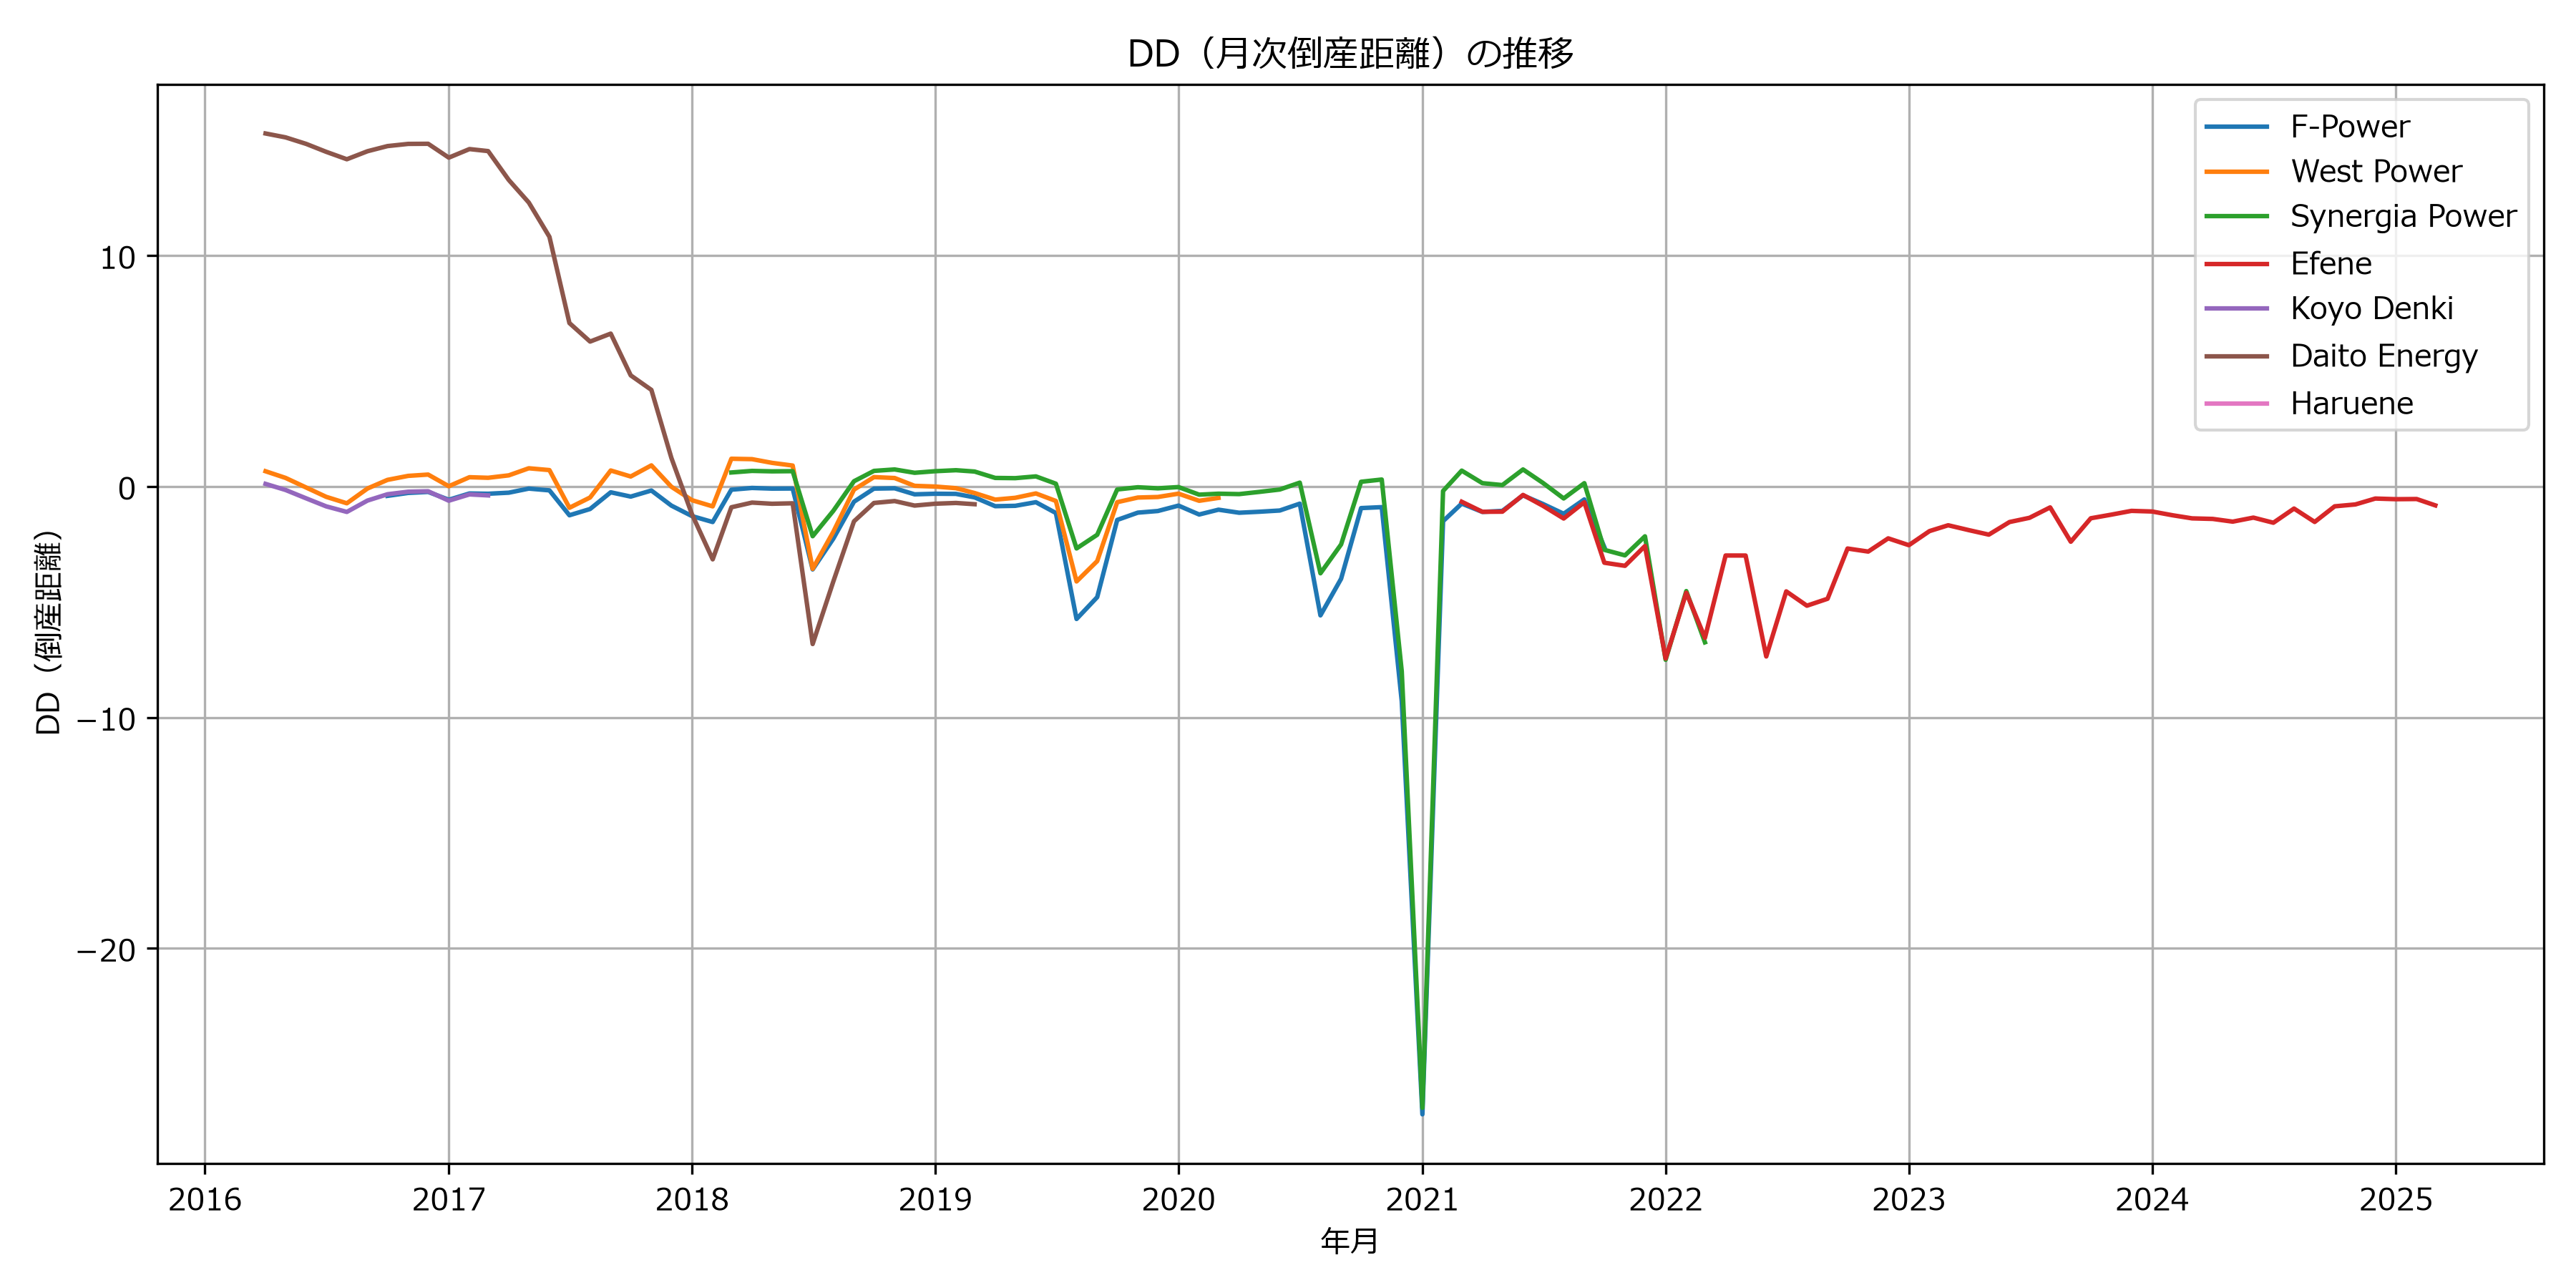
\includegraphics[width=15cm]{Python/figures/dd_monthly_trend.png}
\caption{倒産距離 DD の月次推移（7社）}
\label{fig:dd_monthly_trend}
\end{figure}

% ============================================================
% 6.7 記述統計
% ============================================================

\section{記述統計（7社版）}

主要変数の記述統計を表 \ref{tab:desc_stats_7firms} に示す。

\begin{table}[H]
\centering
\caption{主要変数の記述統計（7社版）}
\label{tab:desc_stats_7firms}
\begin{tabular}{lccccc}
\toprule
統計量 & $\mu$ & $\sigma$ & $D$ & $S$ & default \\
\midrule
count & 359 & 255 & 366 & 306 & 306 \\
mean & 0.022 & 1.462 & 1.050 & 0.000 & 0.000 \\
std & 0.120 & 2.421 & 0.307 & 0.000 & 0.000 \\
min & -0.167 & 0.197 & 0.289 & 0.000 & 0.000 \\
25\% & -0.003 & 0.459 & 0.821 & 0.000 & 0.000 \\
50\% & 0.000 & 0.708 & 1.045 & 0.000 & 0.000 \\
75\% & 0.025 & 1.645 & 1.259 & 0.000 & 0.000 \\
max & 1.800 & 24.147 & 1.937 & 0.000 & 0.000 \\
\bottomrule
\end{tabular}
\end{table}

% ============================================================
% 6.8 本章のまとめ
% ============================================================

\section{本章のまとめ}

本章では，従来の第6章（変数定義と採用根拠）を拡張し，
日本企業 7 社のデータ構築・変数定義・月次補間・倒産距離 DD の計算・記述統計を
すべて統合した。

\begin{itemize}
  \item 収益性 $\mu$，市場ショック感応度 $\sigma$，支援能力 $S$，負債比率 $D$ を
        理論モデルの四要素として実証的に定義した。
  \item 官報公告と JEPX データを統合し，年度データを月次補間して
        倒産距離 DD の月次推移を可視化した。
  \item 記述統計により，変数の分布と新電力企業の財務特性を確認した。
\end{itemize}

これらの処理により，第9章の Ordered Logit 推定に必要な
\texttt{financial\_data.csv} が整備され，
倒産距離 DD の動態を実証的に評価する基盤が完成した。
